\documentclass[a4paper, 12pt]{article}
\usepackage[utf8]{inputenc}
\usepackage[T1]{fontenc}
\usepackage[french]{babel}
\usepackage{graphicx}
\usepackage{amsmath}
\usepackage{amssymb}
\usepackage{graphicx}
\usepackage{float}
\usepackage{hyperref}
\usepackage{geometry}

\geometry{hmargin=1.5cm,vmargin=4cm}
\pagestyle{headings}

\title{Rapport final de Développement Web 2}
\author{Lucas Jouvet, Francis Kempenaers et Tao Grolleau}
\date{\today}

\begin{document}

\maketitle

\begin{abstract}
  Dans ce rapport, nous présenterons le travail effectué pour le projet de Développement Web 2 au cours du semestre 6. Nous décrirons l'application et ses principales fonctionnalités, puis nous expliquerons les différentes technologies utilisées, l'origine du code source. Enfin, nous préciserons quelques détails, tels que le temps investi et le rôle de chacun des membres du groupe.
\end{abstract}

\newpage

\section{Description de l'application}

\subsection{Principales fonctionnalités}

L'objectif de ce projet était de développer un site web d'édition de fichiers en temps réel sur lequel les utilisateurs pourraient communiquer tout en éditant leurs fichiers. Les fichiers sont privés par défaut et visibles uniquement de l'utilisateur qui les a mis en ligne. Il est possible de permettre à d'autres utilisateurs d'éditer les fichiers auxquels on a accès et également de révoquer ces permissions. L'accès au site peut se faire soit par sa page internet dit client léger, soit au moyen d'une application java dite client lourd. Le client lourd présente l'avantage d'intégrer la coloration syntaxique.

\subsection{Différents diagrammes}

\subsubsection{Diagrammes UML}

\begin{figure}[H]
  \begin{center}
    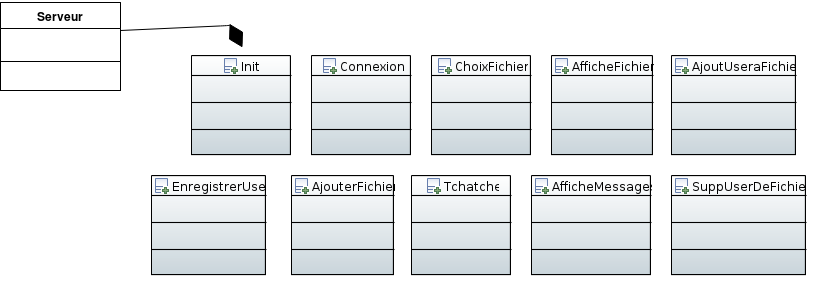
\includegraphics[scale=0.5]{DiagrammeClientLeger.PNG}
  \end{center}
  \caption{Diagramme de classe du client léger}
\end{figure}

\begin{figure}[H]
  \begin{center}
    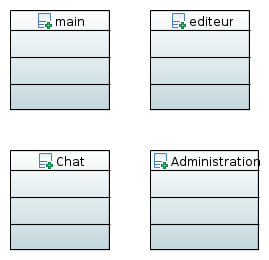
\includegraphics{DiagrammeClientLourd.PNG}
  \end{center}
  \caption{Diagramme de classe du client lourd}
\end{figure}

\begin{figure}[H]
  \begin{center}
    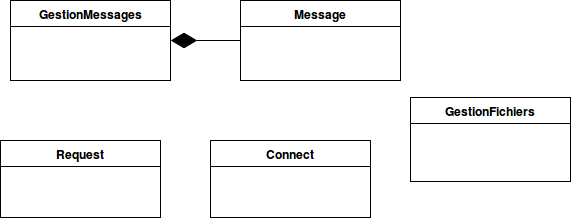
\includegraphics[scale=0.7]{DiagrammeBDD.png}
  \end{center}
  \caption{Diagramme de classe de la base de données}
\end{figure}



\subsubsection{Templates}

\begin{figure}[H]
  \begin{center}
    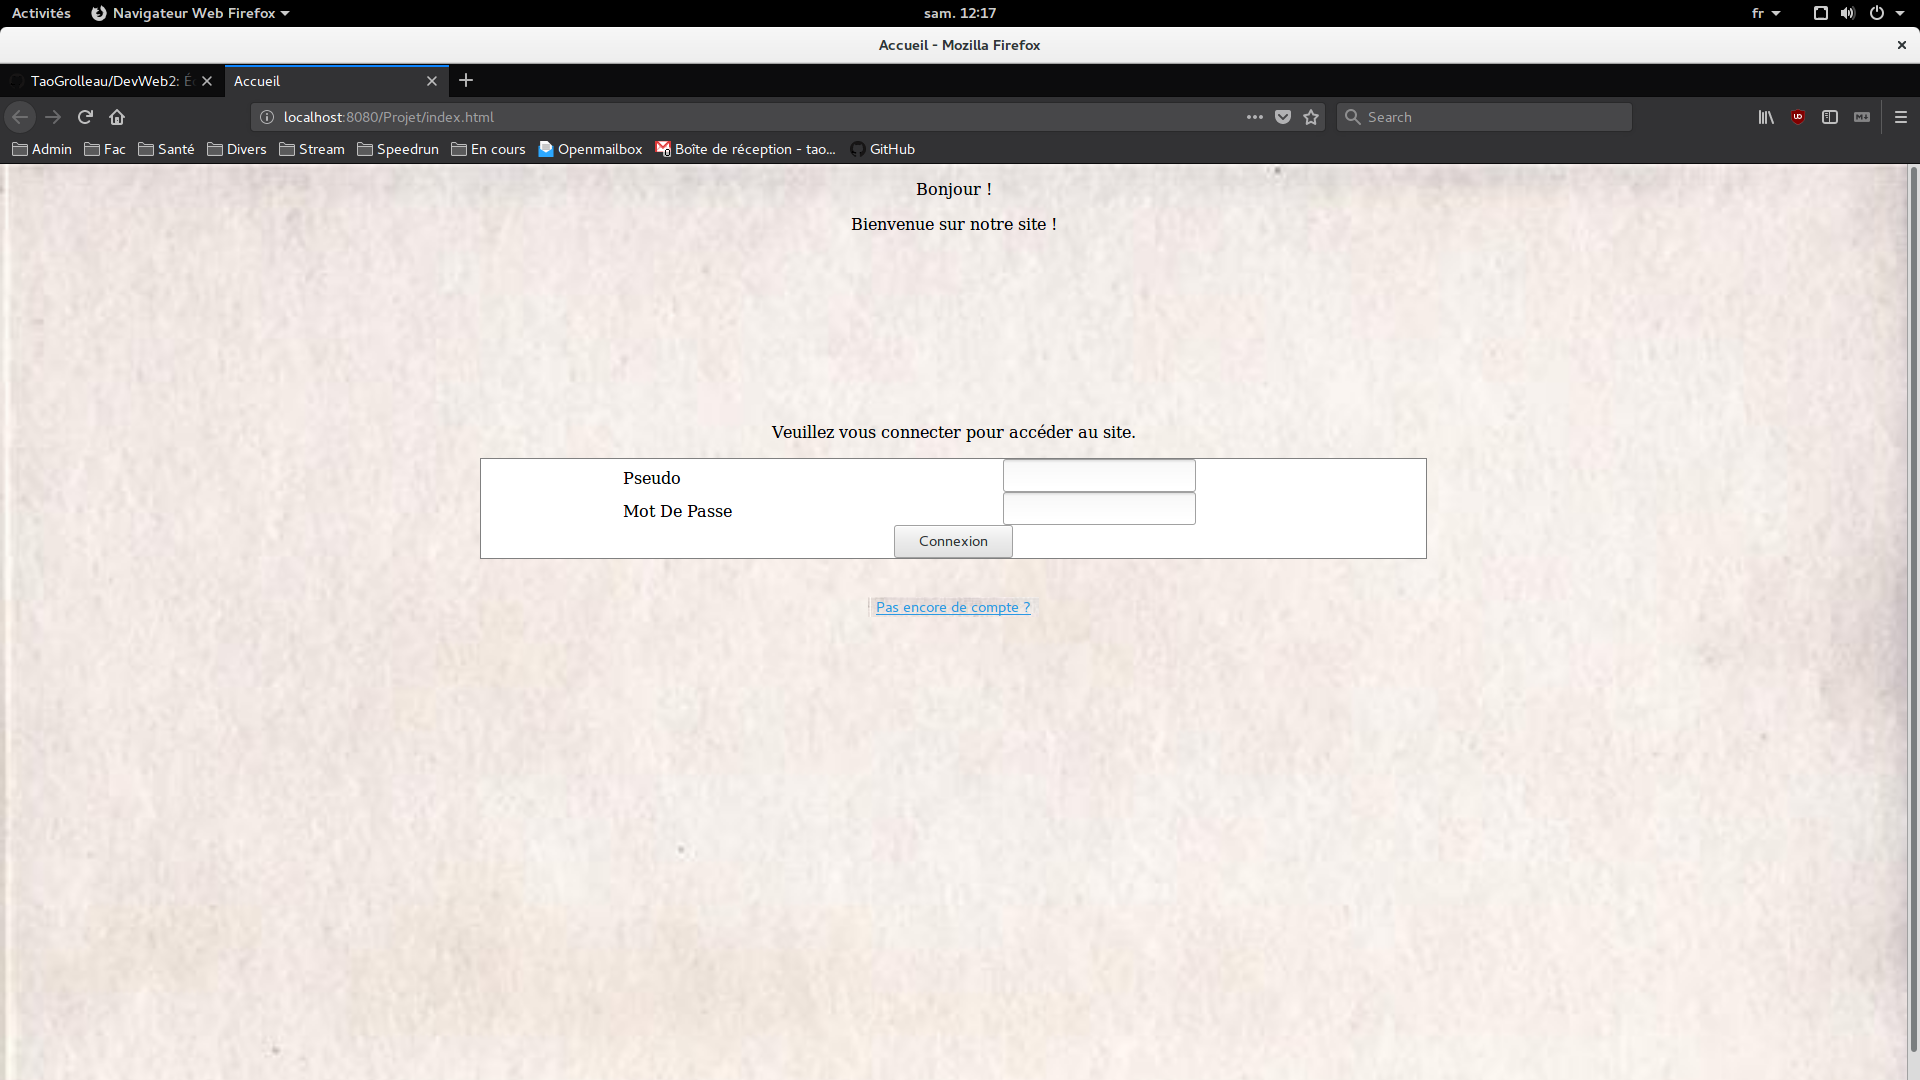
\includegraphics[scale=0.2]{accueil_leger.png}
  \end{center}
  \caption{Écran d'accueil du client léger}
\end{figure}

\begin{figure}[H]
  \begin{center}
    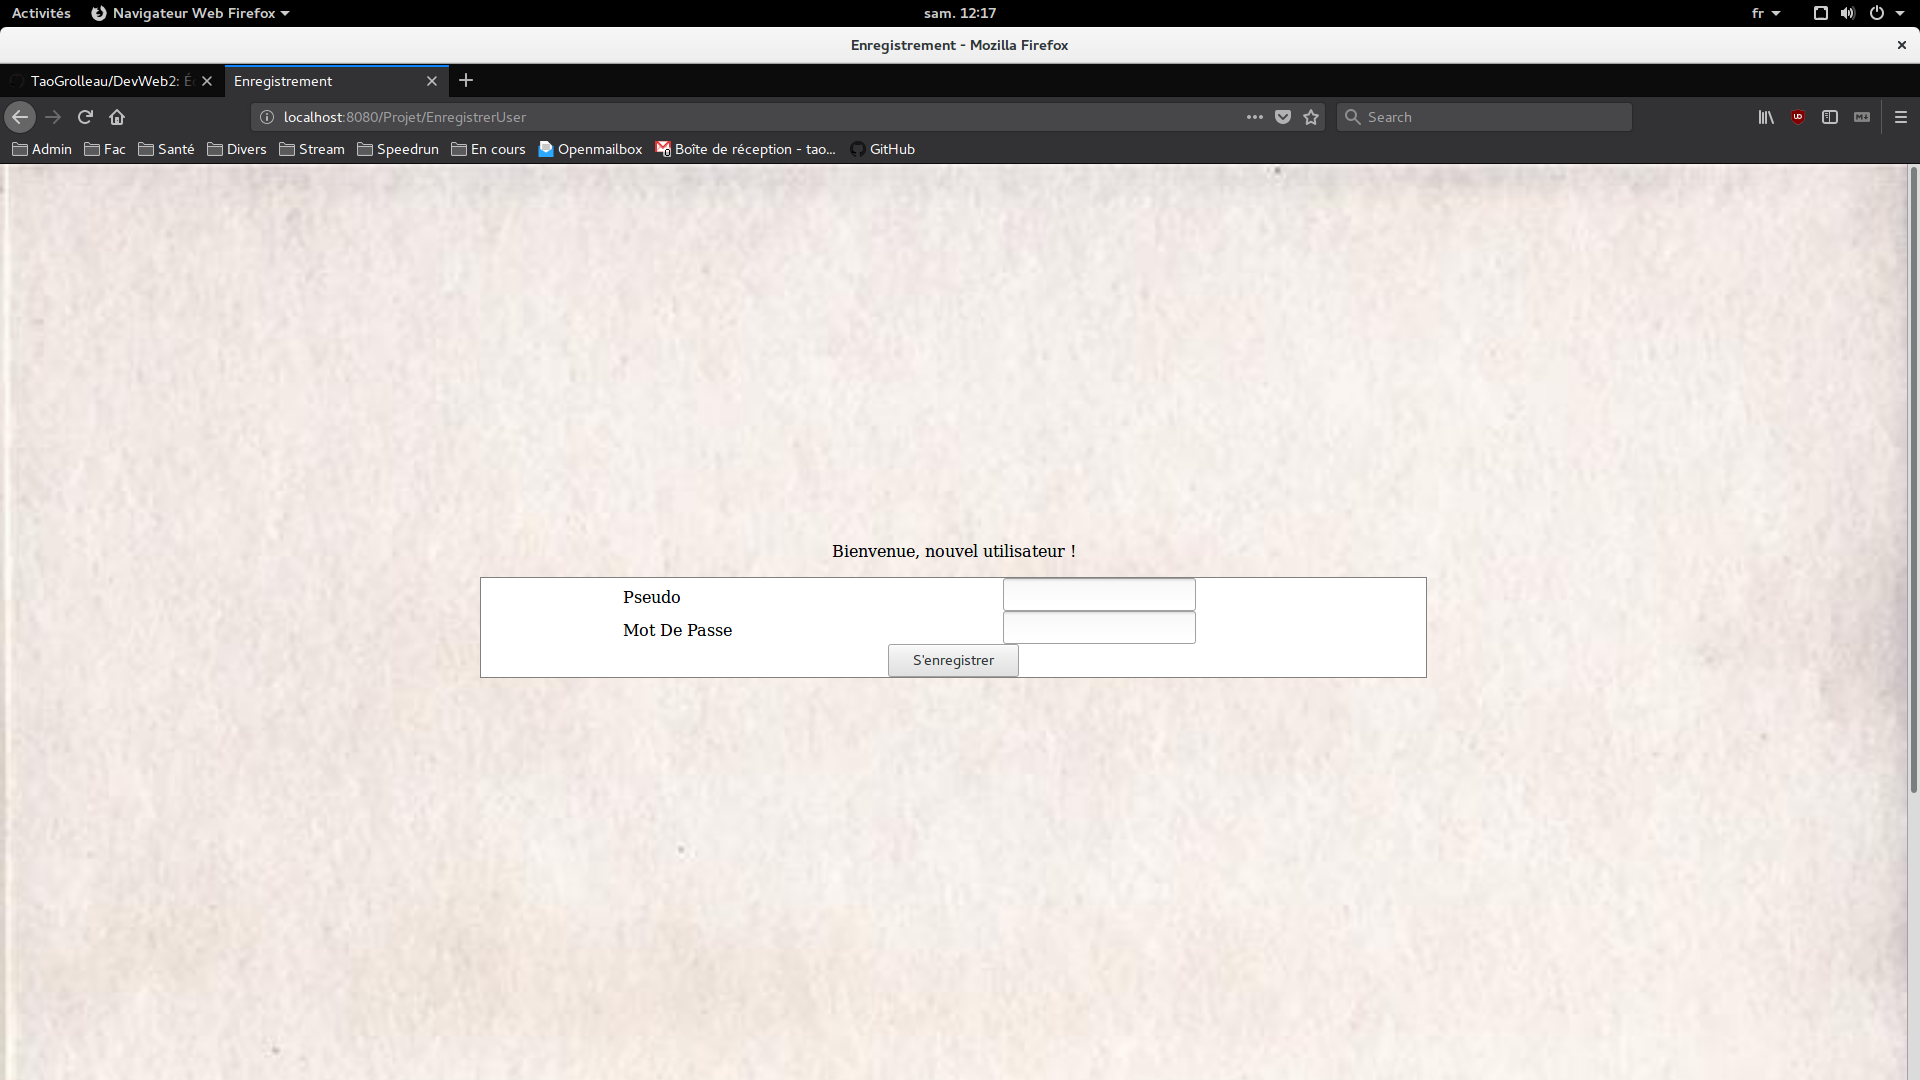
\includegraphics[scale=0.2]{enregistrement_leger.png}
  \end{center}
  \caption{Page d'enregistrement d'un nouvel utilisateur du client léger}
\end{figure}

\begin{figure}[H]
  \begin{center}
    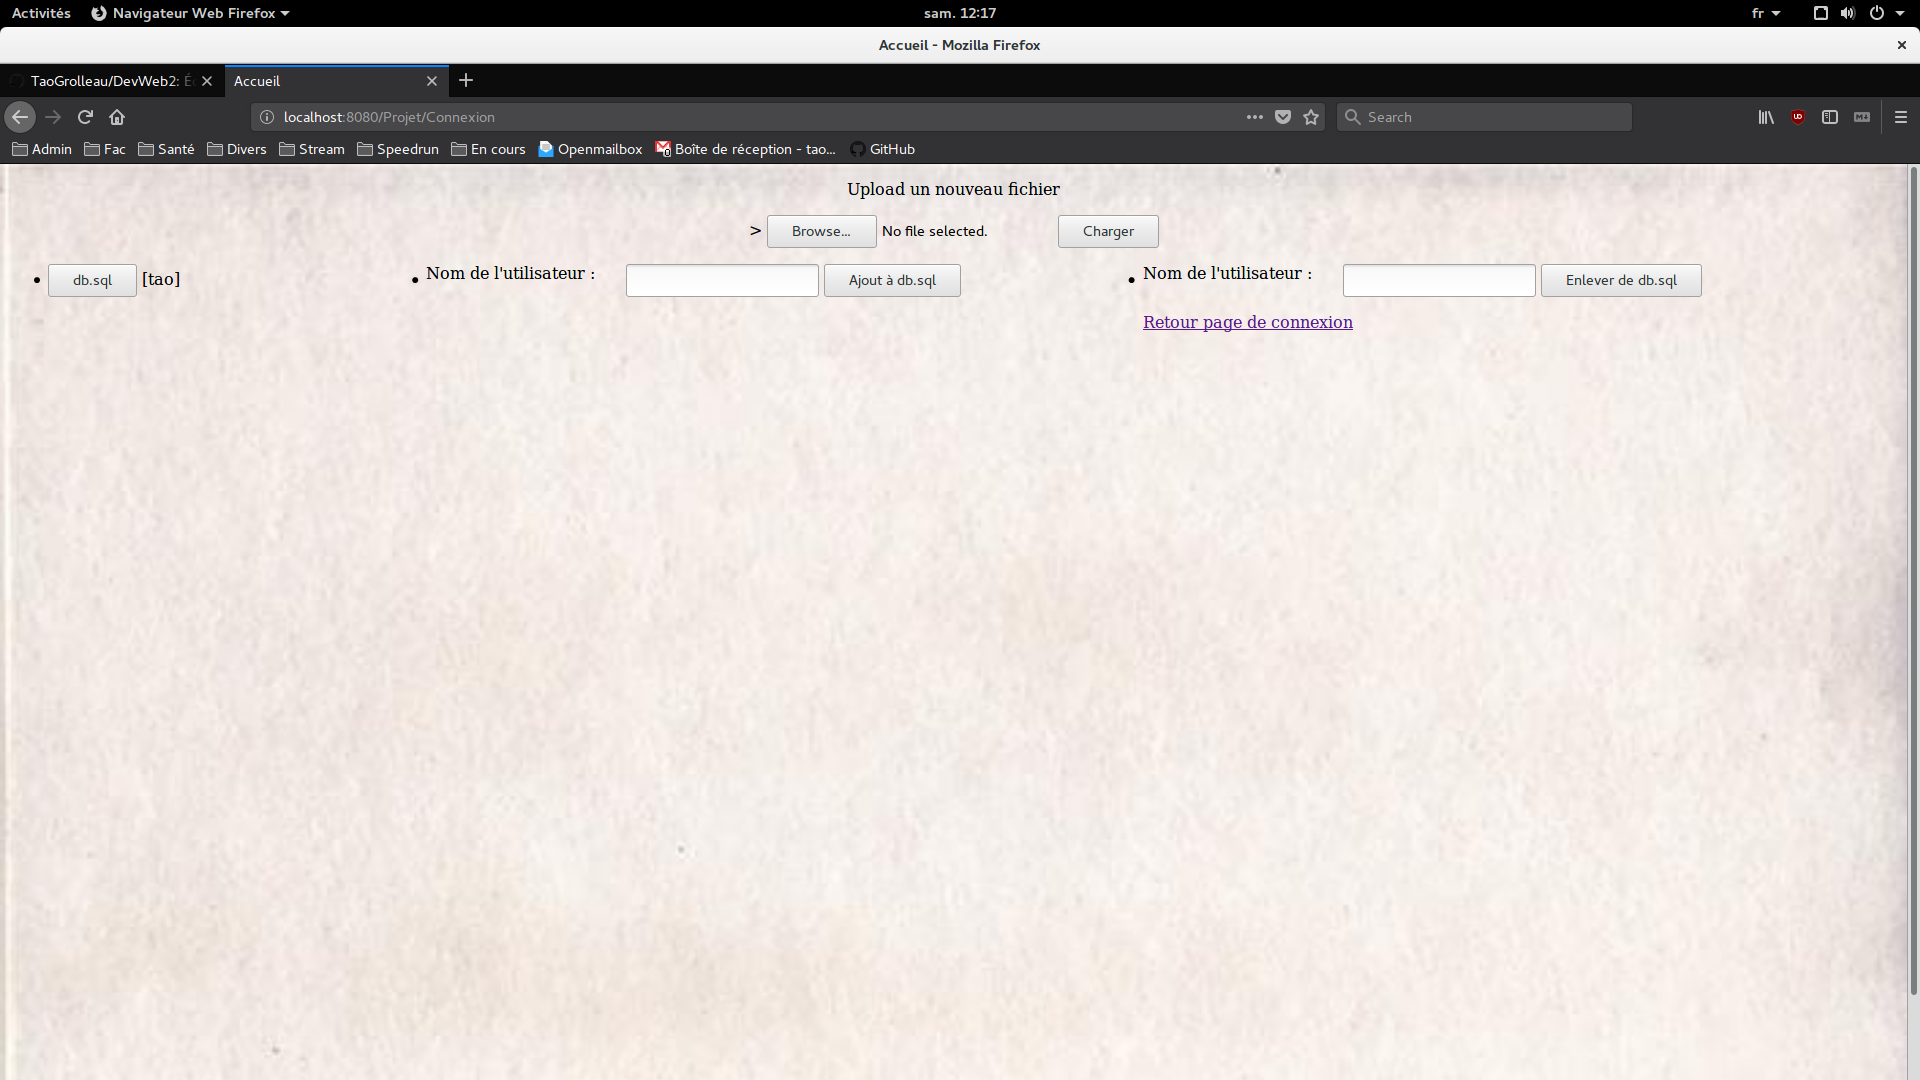
\includegraphics[scale=0.2]{fichier_leger.png}
  \end{center}
  \caption{Liste des fichiers d'un utilisateur du client léger}
\end{figure}

\begin{figure}[H]
  \begin{center}
    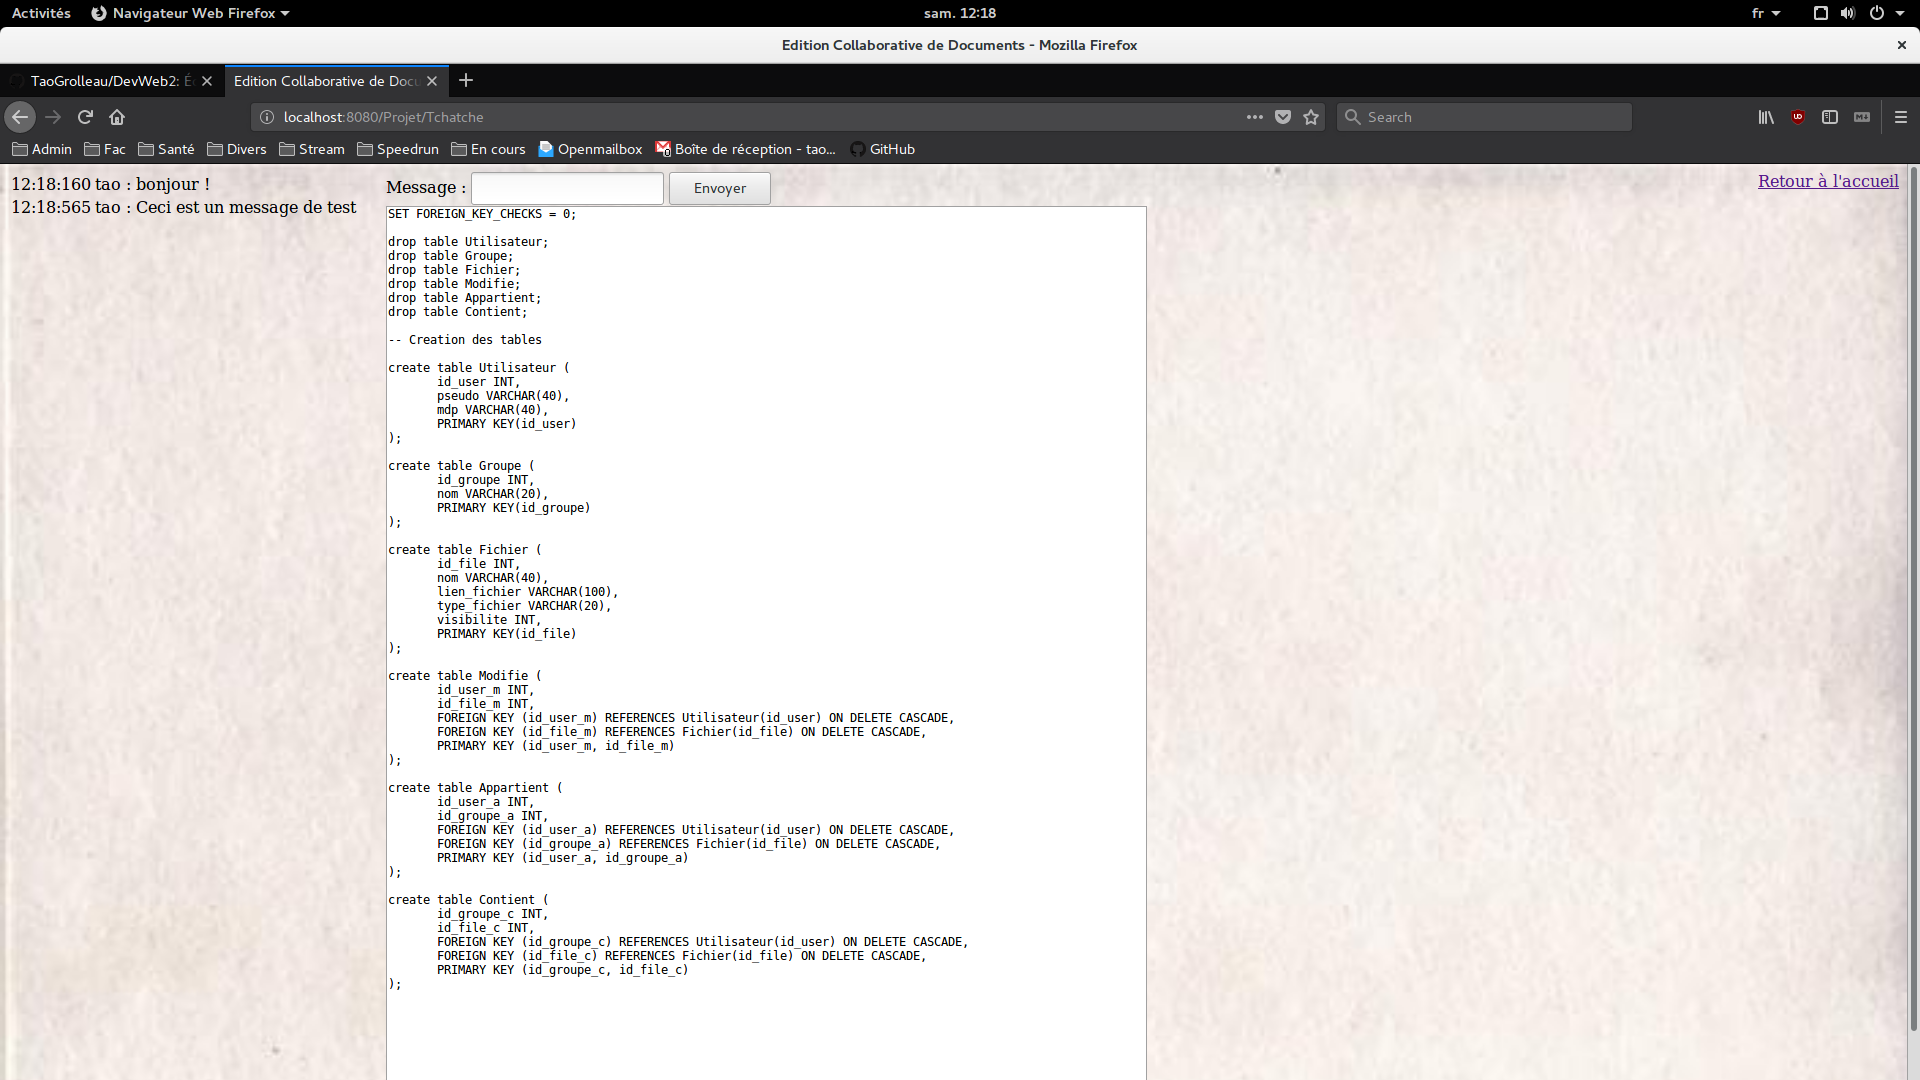
\includegraphics[scale=0.2]{editeur_leger}
  \end{center}
  \caption{Éditeur de fichier et chat du client léger}
\end{figure}

\begin{figure}[H]
  \begin{center}
    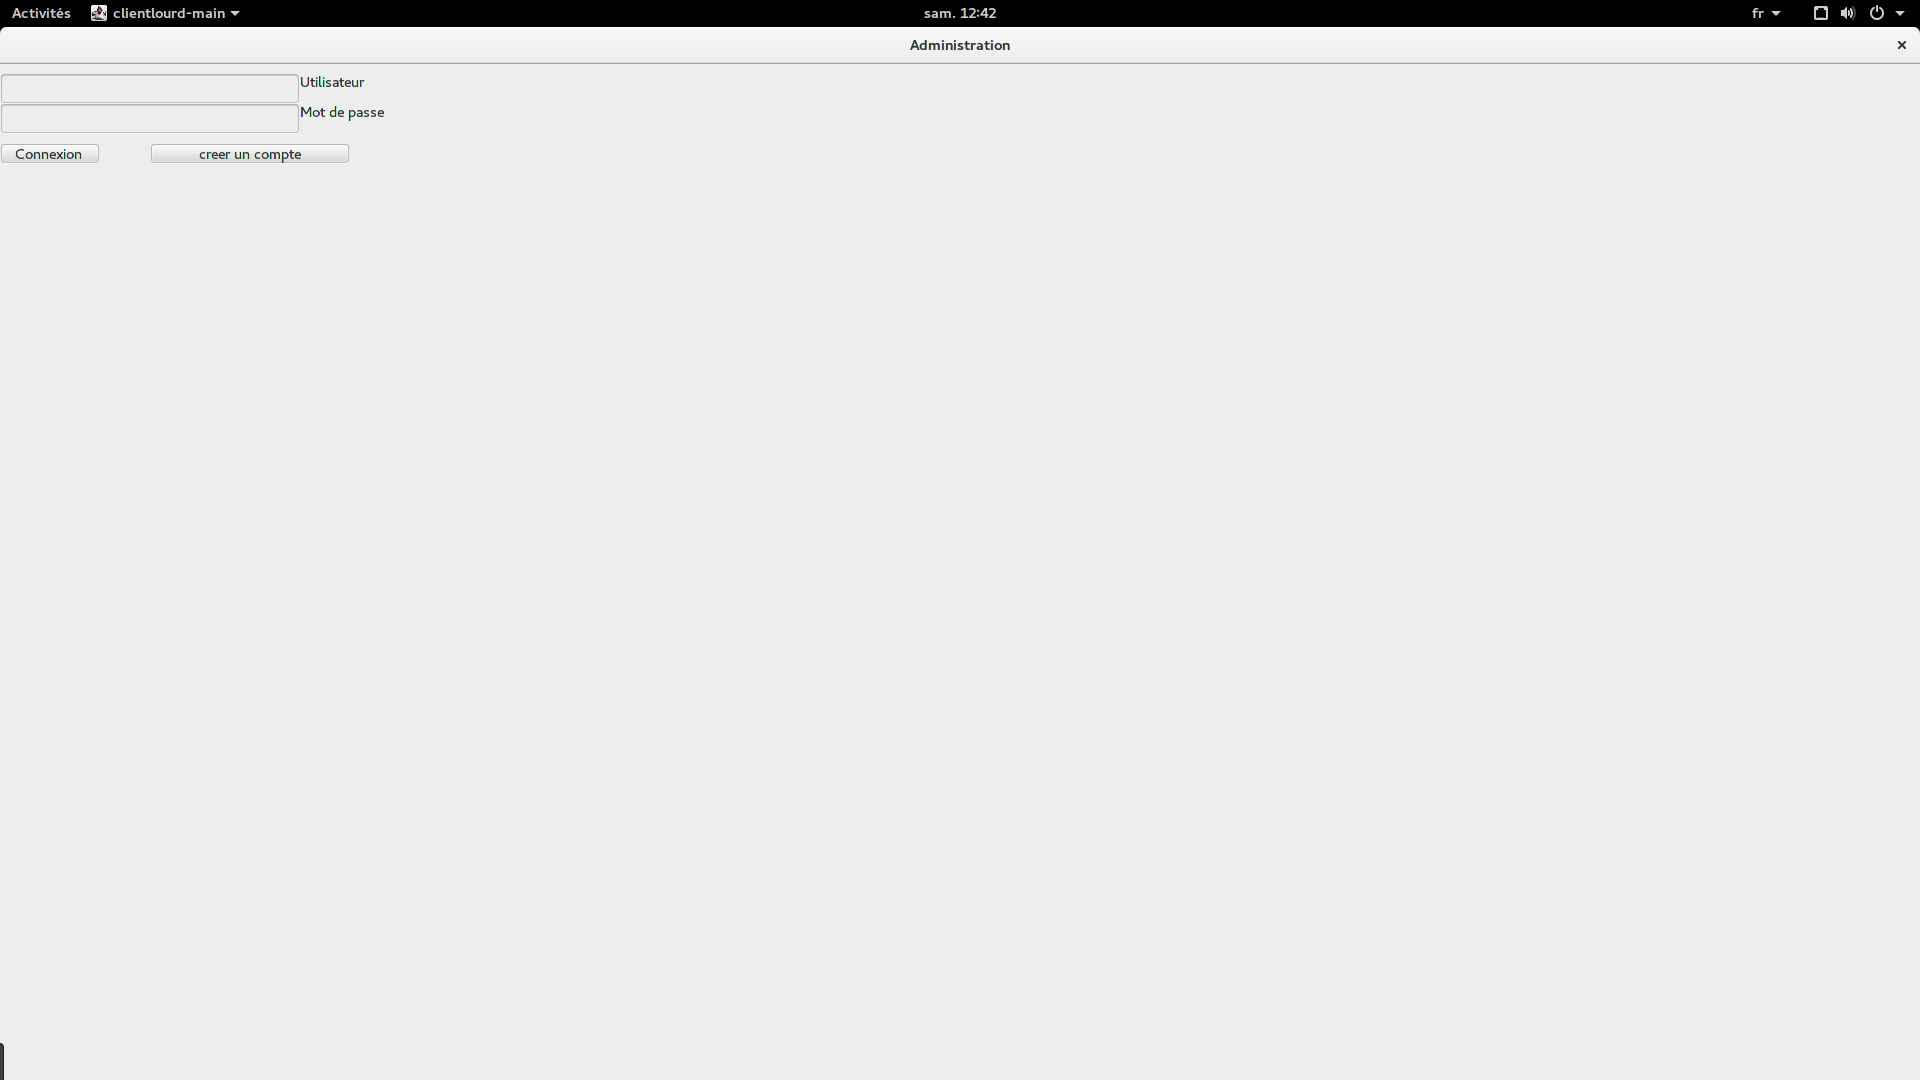
\includegraphics[scale=0.2]{client_lourd.png}
  \end{center}
  \caption{Écran de connexion du client lourd}
\end{figure}

\begin{figure}[H]
  \begin{center}
    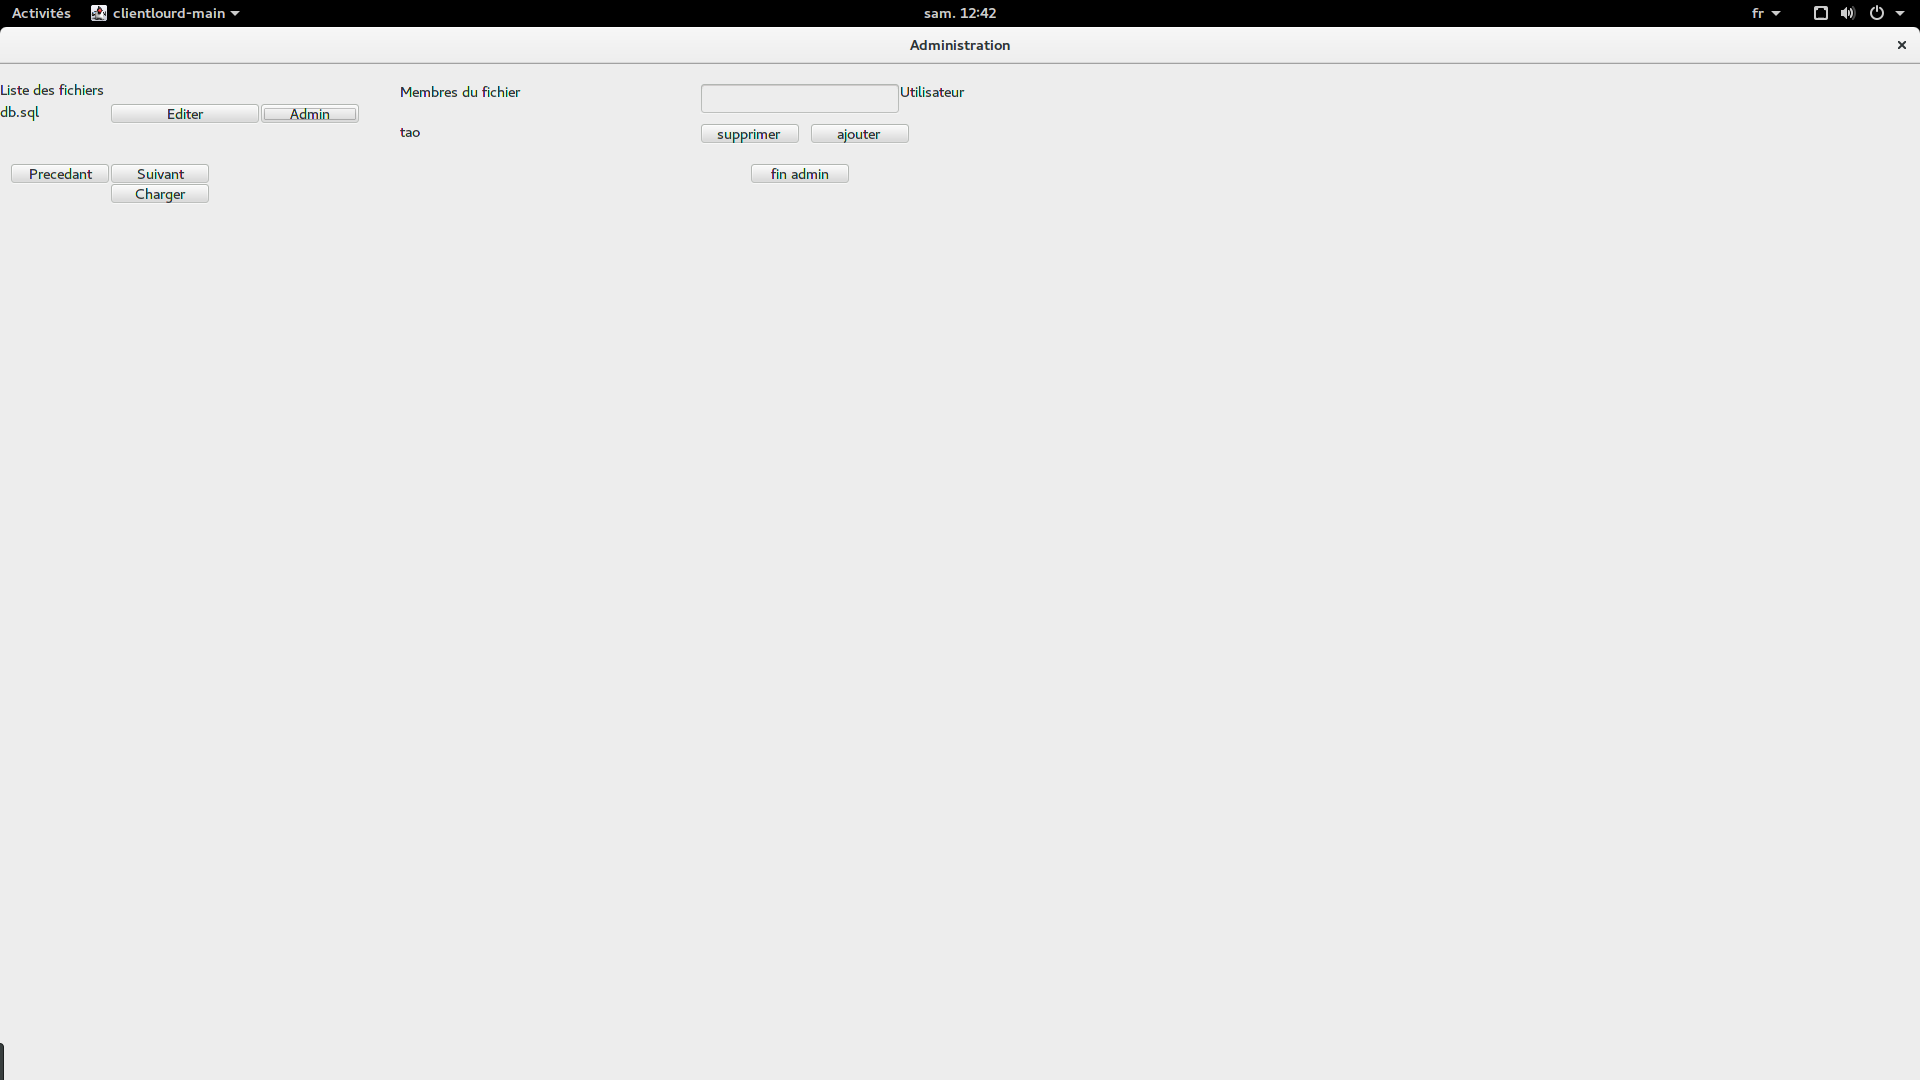
\includegraphics[scale=0.2]{admin_lourd}
  \end{center}
  \caption{Page d'administration du client lourd}
\end{figure}

\begin{figure}[H]
  \begin{center}
    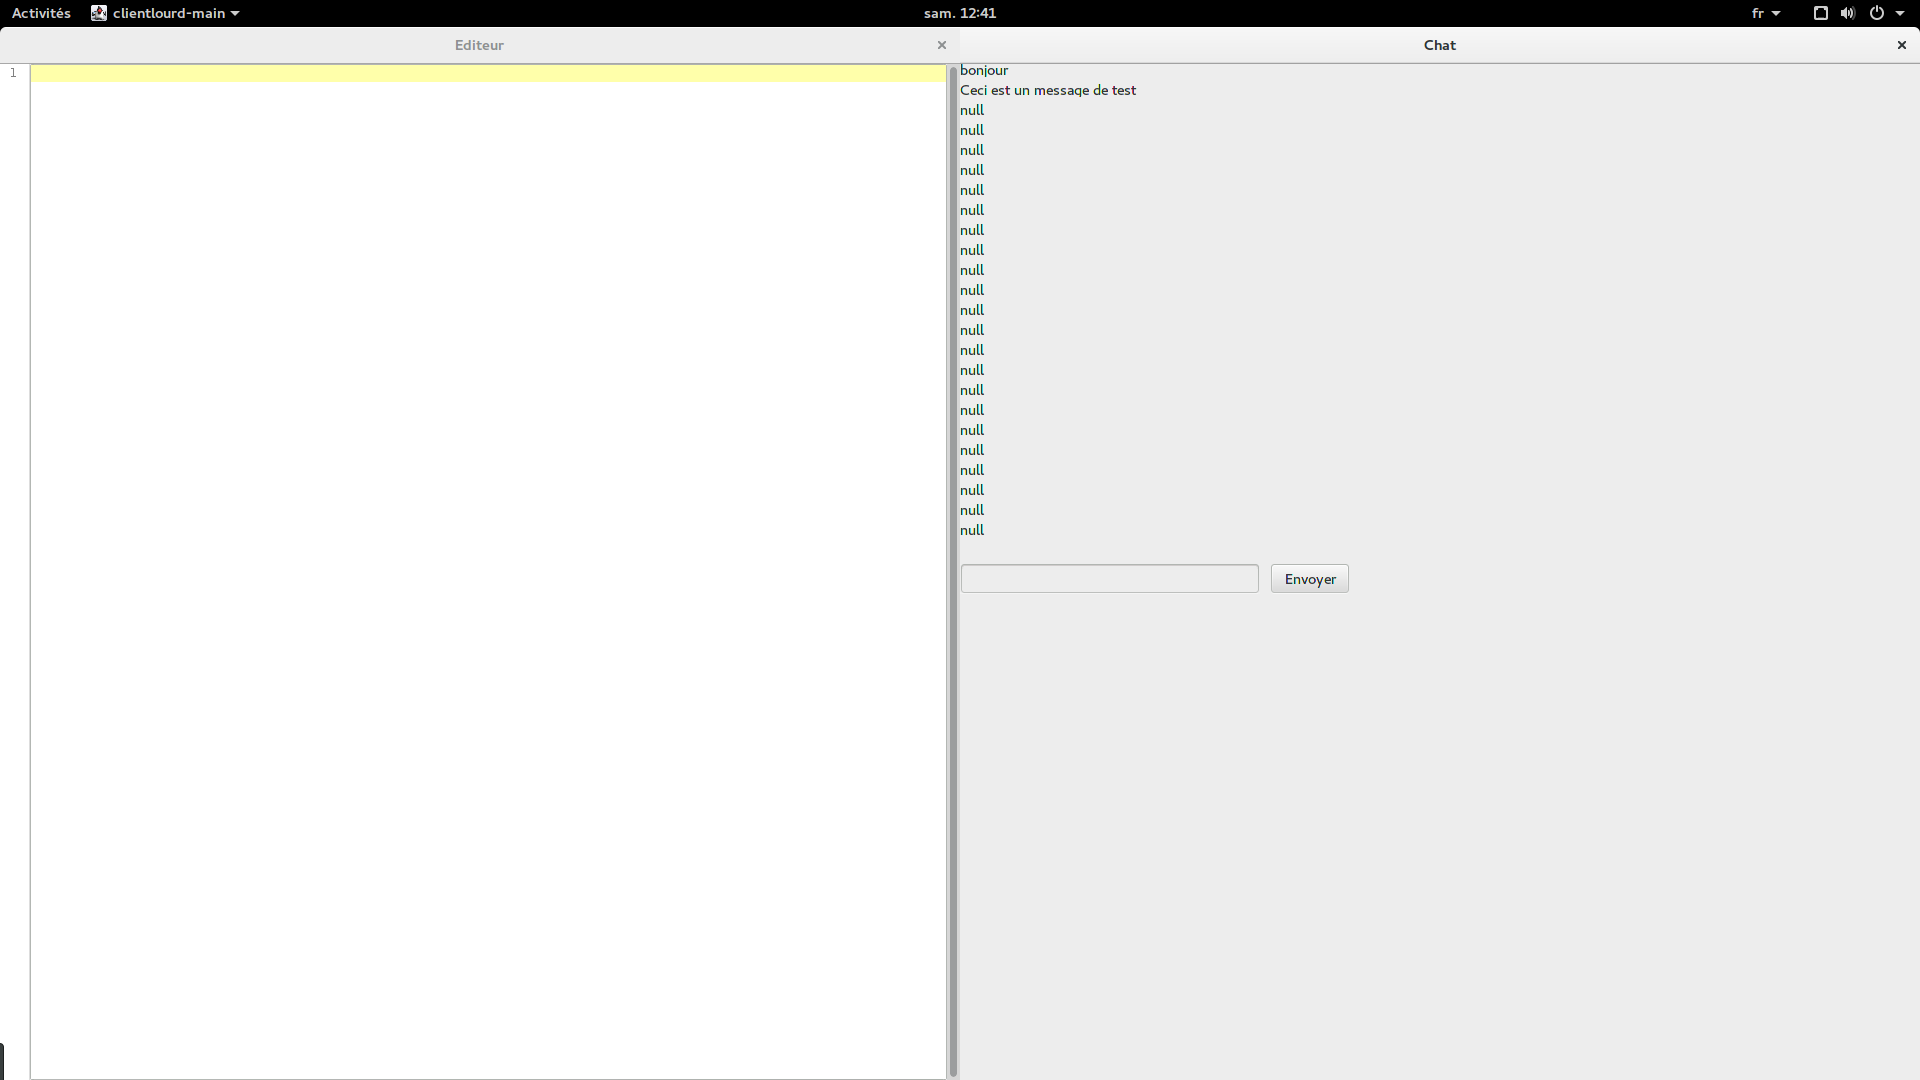
\includegraphics[scale=0.2]{editeur_lourd.png}
  \end{center}
  \caption{Éditeur et chat du client lourd}
\end{figure}


\subsubsection{Schéma Entité-Association}

\begin{figure}[H]
  \begin{center}
    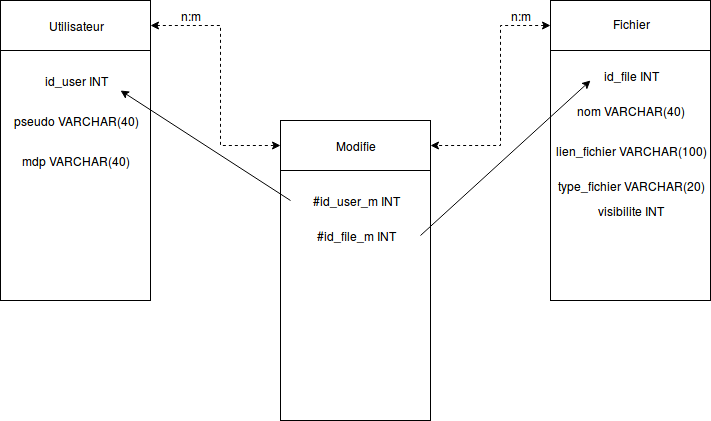
\includegraphics[scale=0.4]{entite_association.png}
  \end{center}
  \caption{Schéma de la Base de Données}
\end{figure}


\section{Technologies utilisées}

Conformément à l'architecture MVC, nous avons utilisé des JSPs comme vues, des servlets comme controlleurs et une classe modèle qui communique avec une base de données mysql. Il va de soit que nous avons eu recours au HTML et au CSS ; le javaScript a quant à lui été utilisé pour permettre la synchronisation des chats et l'édition de fichiers en temps réel. Le client lourd utilise Swing et communique avec le serveur au moyen de sockets.


\section{Origine du code et sources}

À part la classe RSyntaxTextArea récupérée sur GitHub (\url{http://bobbylight.github.io/RSyntaxTextArea/}), le code est entièrement fait à la main. Évidemment, des sites tels que Openclassrooms et StackOverflow ont servi d'aide. La gestion du chat a été largement inspirée de ce qui avait été fait en TP.

\section{Temps investi et rôles des membres du groupe}

Sans avoir pris en compte la durée de chaque journée de travail, nous estimons que nous avons passé tous les trois environ quarante heures chacun sur le projet.
Les rôles ont peu changé, Francis Kempenaers a pris en charge le développement du client léger, Lucas Jouvet, celui du client lourd et Tao Grolleau, la mise en place de la base de données. 

\section{Conclusion}

Bilan critique : Tout d'abord en ce qui concerne l'UE en général, nous regrettons le rythme soutenu (une semaine par notion) qui combiné à la pression des autres UEs ne nous a pas permis d'être aussi performants que nous l'aurions voulu ni d'approfondir le sujet. Le non respect de l'architecture MVC lors des TPs sur les servlets et les JSP a rendu délicat la transition des connaissances du cours vers le projet ou nous devions appliquer cette architecture. L'énoncé du projet est peut être arrivé un peu tardivement même si le gros du travail a été fourni sur la fin du semestre, là encore pour des raisons d'emploi du temps chargé.
\\Concernant notre projet en lui même, nous sommes satisfaits du résultat car l'édition en temps réel nous a donné du fil à retordre ; la fluidité de celle-ci pourrait sans doute être encore améliorée. Une comparaison du rapport intermédiaire au projet final révélera cependant que certaines fonctionnalités (normalement l'édition publique et la boite de messagerie) ont finalement été écartées car nous avions été trop ambitieux au regard du temps imparti. De même, l'interface diffère sensiblement de ce qui avait été prévu pour des raisons pratiques.



\end{document}
